% Axis-body idioms from real documents: two option lists, comparison
% operators, \pgfmathsetmacro before a plot, \pgfplotsinvokeforeach and
% \foreach around plots, a \label after a plot. Behaviour V0.
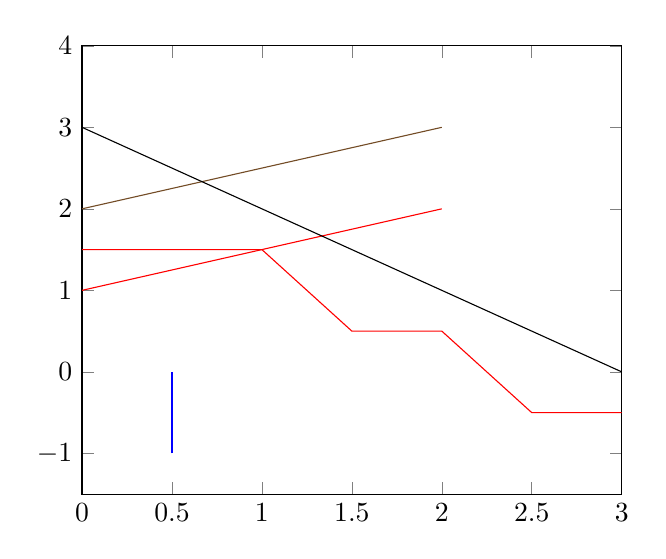
\begin{tikzpicture}
\begin{axis}[xmin=0, xmax=3, ymin=-1.5, ymax=4, samples=7]
  \pgfmathsetmacro\offset{0.5}
  \addplot [red] [domain=0:3] {(x<=1)*1 + (x>2)*(-1) + \offset};\label{pl:step}
  \pgfplotsinvokeforeach{1,2}{
    \addplot+[domain=0:2, samples=3, mark=none] {x/2 + #1};
  }
  \foreach \k in {3} {\addplot+[domain=0:3, samples=2, mark=none] {\k - x};}
  \draw[blue] (axis cs:\offset,-1) -- (axis cs:\offset,0);
\end{axis}
\end{tikzpicture}
